\documentclass[letterpaper, 12pt]{article}
\usepackage[letterpaper, portrait, margin=1in]{geometry}
\usepackage{multicol}
\usepackage[english]{babel}
\usepackage{graphicx}

\usepackage{xcolor}
\usepackage{blindtext}

% Paper requirement 1.5 line spacing. Remove for github publishing
\usepackage{setspace}
\onehalfspacing

\title{Automatic Singing Transcription}
\author{Victor Shan}
\begin{document}
\maketitle
\begin{multicols*}{2}
\begin{abstract}
\end{abstract}

\section{Introduction}

Songs play an important part of society because they are conduits of cultural expression,
foster emotional connection and is a great source of entertainment. Automatic Singing Transcription
(AST) is a branch of Automatic Speech Recognition (ASR) can facilitate a deeper way to interact with
it. In ASR, the goal is to transcribe normal speech to text,
whether that's a conversation between two people, a lecture, or a podcast. Examples of ASR include
Youtube's auto-generated captions, assistants like Siri and Alexa, and even live captioning of
meetings through applications like Zoom. AST is a similar task, but instead of transcribing normal
speech, AST transcribes singing. Applications of AST range from karaoke applications to Music
Information Retrieval (MIR) systems. These MIR systems can be used to search for songs based on
lyrics, categorize songs based on their lyrics, or even aid in the generation of new songs.

While AST is similar to ASR, there are a few key differences that make it a more challenging task.
First, singing is a more complex signal than normal speech. Singing has a more dynamic signal, with
more variation in pitch, duration and vibrato \cite{SemiSupervisedSolo}.
For example, vowels sounds are often held for longer in singing than in normal speech like dragging
the last part of ``bye" in word ``goodbye". Songs also often include music in the background, which can
make it more difficult to distinguish between the singer's voice and the background music. Finally,
there is a lack of large, publicly available datasets for AST \cite{DALI}. This is in contrast to ASR, where
there are many large datasets available, such as LibriSpeech \cite{Librispeech}. This lack of data
makes it especially difficult to train AST models.

There are many possible outputs for AST but one of the most detailed and useful outputs is the
time-aligned phoneme sequence. This is a sequence of phonemes, or the smallest unit of sound in a
language, that is aligned with the audio. Time-aligned phoneme sequences are useful because it can contains enough
information to reconstruct the not only the lyrics, but also how they match with the music. This
output can be used to generate a karaoke application that highlights the lyrics as they are sung,
or even train a model to sing covers of songs. Word-level alignement is an easier alternative but it
misses the crucial information of the duration of phonemes within words. The ideal output is one that includes even more information
such as the notes to sing at so that singers would be able to read and sing the song without any
additional information. In this paper, we will mainly focus on the phoneme-level alignment but use
word-level alignment to compare the performance of our model to other models.


\section{Datasets}

\subsection{Requirements}
The requirements of a good dataset are audio files, lyrics and timestamps. The audio files can be
in any format such as mp3 or wav. The lyrics can be in any format as well, but the timestamps must
be in a format that can be used to align the lyrics with the audio. The timestamps can be in the
form of a phoneme sequence or word sequence but should also include the onset and offeset times
(beginning and end). Sentence level timestamps are too coarse and would need
to be broken down into word or phoneme level timestamps. Most lyrics used by popular music services
such as Spotify only use sentence/line level timestamps. Ideally, the dataset would also be large
enough to train deep neural networks and publicly available so that other researchers can use it and
compare their models to existing models.

\subsection{Challenges}
With these requirements in mind, it is easy to see why there are so few datasets available. First,
it is difficult to create a dataset with lyrics and timestamps. The lyrics must be manually
transcribed and the timestamps must be manually aligned with the audio. This is a time consuming
process that requires a lot of effort. Second, it is difficult to obtain the rights to use the
audio files. Most songs are owned by record labels and it is difficult to obtain the rights to use
these files. These two challenges make it difficult to create new datasets and is the reason why
there are so few datasets available and why most of the existing datasets are small.

\subsection{Dataset Augmentation}
\subsubsection{SpecAugment}
Due to the lack of datasets, it is more important to make the most of the existing datasets. One
way to do this is to augment the existing datasets. SpecAugment is a series of techniques that
augment the audio spectrogram to improve the performance of ASR models. A frequent intermediate
representation are Mel-Frequency Cepstral Coefficients (MFCC). These are image representations of
energy at certain frequencies on a scale that more closely matches human hearing \cite{MFCC}.
These techniques include time warping, frequency masking and time masking \cite{SpecAugment}.
Time warping is a technique that stretches or compresses the audio spectrogram in the time
dimension. Frequency masking is a technique that masks a random number of frequency channels in
the audio spectrogram. Time masking is a technique that masks a random number of time steps
in the audio spectrogram. These techniques are used to augment the audio spectrogram before it
is fed into the ASR model. \cite{SpecAugment}

% ----------------- INCLUDE MFCC IMAGE -----------------

\subsubsection{Transforming Existing Datasets Into Pseudo-Singing Datasets} \label{sec:pseudoSinging}
Another way to augment the existing datasets is to transform the existing datasets. This can be
done by shifting the pitch, duration or vibrato \cite{SongifiedSpeech}. The advantage of this
technique is that is can also be applied to speech datasets and transform them into pseudo-singing
datasets. The disadvantage is that the results will contain artifacts from the transformation based
on the techiniques applied. Neural network models showed an almost 15\% improvement on the
transformed TIMIT dataset than ones trained on the original TIMIT dataset \cite{SongifiedSpeech}.

\subsubsection{Transforming Utterance level datasets into Phoneme level datasets} \label{sec:utteranceToPhoneme}
A technique from ASR that can also be applied to AST is transforming utterance/sentence
level datasets into phoneme level datasets. There are many ASR datasets that contain single utterances
such as LibriSpeech and MUSDB18 \cite{Librispeech,musdb18}. These datasets can be effectively
transformed into phoneme level datasets by using a phoneme dictionary such as the CMU Pronouncing
Dictionary \cite{CMUDict}. This dictionary contains a mapping from words to phonemes. Using this
dictionary, the utterances can be transformed into phoneme sequences. These sequences can then be
used with a Connectionist Temporal Classification (CTC) loss function to train AST models \cite{CTC}.
\begin{figure*}
    \centering
    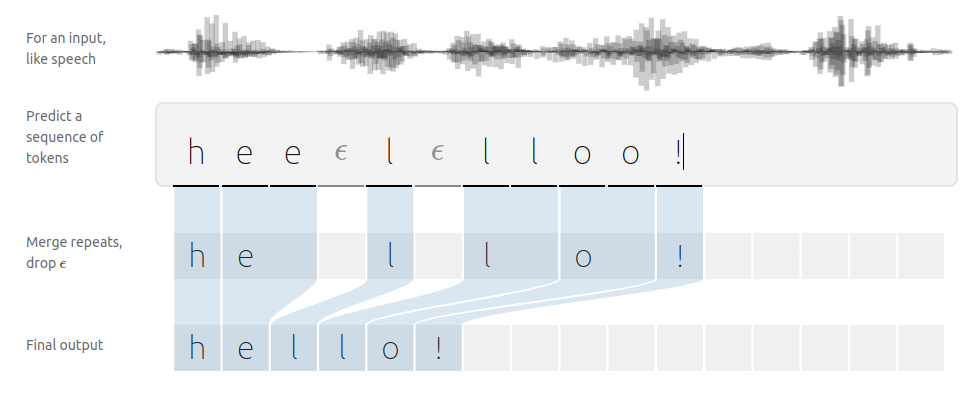
\includegraphics[width=0.5\textwidth]{assets/CTC.png}
    \caption{CTC Function collapsing repetitions \cite{CTC}}
    \label{fig:CTC}
\end{figure*}
CTC allows for the model to output a sequence of phonemes per time step and the
repetitions are collapsed into a single phoneme as shown in Figure \ref{fig:CTC}.
This technique was used to allow a model to incorperate the utterance level LibriSpeech
dataset into the training for a phoneme ASR model \cite{wav2vec}. Timestamps can be
retrieved from the pre-CTC output that had time-aligned phoneme classifications.
The same process can be applied to AST models to allow them to use the utterance level song datasets.

\subsubsection{Teacher-Student Approach} \label{sec:TeacherStudent}
The teacher-student approach is inspired by the technique of the same name that was intended
to reduce the size of large deep neural networks. The idea was first train a large deep neural
network, the teacher, and then train a smaller deep neural network, the student, to mimic the
teacher \cite{TeacherStudent}. However, this technique can also be applied in cases of low labeled
data availablility but high unlabeled data availablility. To start off, a model would be
trained on a small dataset of labeled data. Then, the model would be used to label a large dataset
of unlabeled data. Finally, a new model would be trained on the newly labeled dataset
\cite{DALI}. This has proven to be effective for transcribing drums in music with the student
model outperforming the teacher model \cite{DrumsStudentTeacher}.

\subsection{Existing Datasets}

\subsubsection{TIMIT (ASR)}
TIMIT is a dataset of speech recordings of 630 speakers of eight major dialects of American English
with time-aligned phoneme sequences \cite{TIMIT}. It is a popular dataset for ASR and has been used
to train many ASR models. However, since this is not a singing dataset, it does not contain any of
the characteristics of singing such as pitch, duration or vibrato. This is an excellent dataset to
apply transformation into a pseudo-singing dataset metioned in \ref{sec:pseudoSinging}. The popularity of this dataset
makes it a good candidate for applying transformations to create a pseudo-singing dataset and also
for a general benchmark to compare against other models.

\subsubsection{LibriSpeech (ASR)}
LibriSpeech is a 1000 hour dataset of audiobook recordings where each recording has a matching sentence \cite{Librispeech}. This
dataset is also a popular dataset for ASR and has been used to train many ASR models including
recent breakthroughs like wav2vec 2.0 \cite{wav2vec}. This dataset is also a good candidate for
training AST models because it is large and publicly available. This dataset is special because of
the clarity of the audio and previous success by other models such as the wav2vec 2.0 model in
detecting phonemes in this dataset when fine tuned with the TIMIT dataset \cite{wav2vec}. This is
done through the CTC technique mentioned in \ref{sec:utteranceToPhoneme}. Since
speech and singing both use the same phonemes, because they are in the same language, this large
dataset can be used to train base models before fine-tuning them AST models.

\subsubsection{Jamendo Dataset}
This dataset one of the most popular datasets for AST and has been used by many state-of-the-art
AST models. It contains 20 English songs and 60 songs in other languages with word-aligned timestamped sequences \cite{JamendoLyrics}. This dataset
is a good candidate for training AST models because it is publicly available and it's popularity
makes it an excellent benchmark to compare against other models. However, it is still a relatively
small dataset and does not contain any phoneme sequences. The authors of this dataset were able to
achieve a 77.8\% Word Error Rate (WER) which still leaves a lot of room for improvement.
{
\color{red}
Remember to record the performance of the state of the art models on this dataset
}
% \subsubsection{Children's Songs Dataset} All Korean :(
\subsubsection{MUSDB18}
MUSEDB18 is a dataset of 150 songs with isolated vocals and accompaniment tracks \cite{musdb18}. This
dataset is a good candidate for training AST models because it is publicly available and it has
clean isolated vocals. The downside of this dataset is that it doesn't contain any word level
timestamps. However, with the CTC technique mentioned in \ref{sec:utteranceToPhoneme}, this dataset
can still be used to train AST models.

\subsubsection{NUS Dataset}
This dataset is one of the few datasets that contains phoneme level timestamps \cite{NUSDataset}.
There are 169 minutes of 20 unique English songs by 12 different people. The CMUDict was used
for the phoneme vocabulary and timestamps were manually annotated. This dataset is the ideal dataset
type for training AST models due to this level of detail. It also includes a mix of slow to fast
melodies annd a balanced gender distribution \cite{NUSDataset}.


\subsubsection{Free Music Archive}
The Free Music Archive (FMA) dataset is a dataset of 106,574 tracks with 161 genres \cite{FMA}. This
dataset is not a good candidate for direclty training AST models because it does not contain any lyrics
and some music may not even contain any singing at all. However, it is a good source of unlabeled
songs that could be labeled through the teacher-student technique in \ref{sec:TeacherStudent}. It
can also provide a good source of general singing audio that can be used in the
training of wav2vec2.0 models that will be described in section \ref{sec:wav2vec}.

\subsubsection{VocalSet}
VocalSet is a 10 hour dataset of a capella singing from 20 professional singers
demonstrating a variety of singing techniques \cite{VocalSet}. This dataset is a good candidate for
training Voice Activity Detection (VAD) models because it contains onset and offset timestamps for
each vocal segment. This is also a good a good dataset to help train AST models to know what singing
sounds like.

\subsubsection{Other Datasets}
Many datasets were considered but left out due to the lack of availablility. Some of the most
popular datasets such as Mauch's Dataset \cite{mirex2021} and Hansen's Dataset \cite{Hansen} are
not publicly available anymore. Newer datasets such as DALI \cite{DALI} and DAMP! \cite{DAMP} are
are hidden behind institutional logins and require manually requesting access.

While both the Mauch's Dataset and Hansen's Datasets are quite small (Mauch has 20 songs, Hansen has 9 \cite{mirex2021}), the
DALI and DAMP! datasets are much larger. The DALI dataset in particular used a version of the
Teacher Student technique mentioned in \ref{sec:TeacherStudent} to label 105 songs with timestamps
for the word and phoneme level \cite{DALI}. The DAMP! dataset is even larger with 300x30x2 song
dataset. Both of these datasets would be excellent candidates for training AST models from their
size alone.

\section{Related Works}
\subsection{HMM Based Acoustic Models}
The traditional approach to AST is can be separated into a pipeline of distinct steps. The first
step is to extract the features from the audio. This usually includes some form of spectral analysis
such as MFCCs. The second step is to use an acoustic model to classify the features into phonemes
and generate a sequence of phonemes using a Hidden Markov Model (HMM). This is the traditional
approach to ASR and is also used in AST \cite{Hansen}.

{
\color{red}
TODO: Add more detail about HMMs
TODO: Write about Dynamic Time Warping
TODO: Write about some results of HMMs
}

% \subsection{Music Informed Models}

\subsection{wav2vec 2.0 and Transfer Learning} \label{sec:wav2vec}

\subsubsection{wav2vec 2.0}
One of the most recent breakthroughs in ASR is wav2vec 2.0 \cite{wav2vec}. This model uses a
self-supervised learning approach was used during the training of the model. Unlabeled audio was
fed into the model to learn discrete speech units. These discrete speech units required the
Gumbel-Softmax \cite{gumbelSoftmax} to allow for backpropagation. The model was then
fine-tuned with a linear layer and CTC loss on labeled data to perform ASR \cite{wav2vec}.

This approach was able to achieve state-of-the-art results on the LibriSpeech dataset \cite{Librispeech}
and the TIMIT dataset \cite{TIMIT}. However, the thing that makes this approach the most promising
is the fact that after pre-training on a large amount of unlabeled data, the model can be fine-tuned
on a 10 minute subset of labeled data to achieve 5.2 WER on the LibriSpeech clean dataset \cite{wav2vec}.
This is very important for AST because there are so few labeled datasets available.

\subsubsection{wav2vec 2.0 Transfer Learning}
Using transfer learning for AST using wav2vec 2.0 was attempted in 2022 and was used to achieve
state-of-the-art results on the Jamendo dataset as well as on the DALI, Hansen, Mauch,
and DAMP! datasets \cite{wav2vecTransfer}. The approach they performed did not change the first part
of the model that generated the discrete speech units. Instead, they changed the last part of the
model to have another branch that outputs the probability of the current word given previous words
and context. This approach achieved a 33.13 WER on the Jamendo dataset \cite{wav2vecTransfer}.

Apart from their results, there were also a few other interesting things about their approach. Since
the initial wav2vec 2.0 model was trained on the LibriSpeech dataset, they wanted to make the input
audio of their model as similar to the LibriSpeech dataset as possible. To do this, they used
Demucs v3 \cite{Demux} to separate the vocals from the accompaniment. They did not futher remove any
noise or singing specific features from the audio. For their labeled datasets, they used
utterance level labels excluding the instrumental parts. For the output, they used character level
labels.


\subsection{Whisper Word-Level Alignment}

\section{Method}
\begin{enumerate}
    \item Preprocess datasets
    \item Augment datasets
    \item Create frankenstein dataset
    \item Train model
    \item Evaluate model
    \item Label unlabeled datasets
    \item train student model on newly labeled datasets
    \item evaluate student model on original, manually labeled datasets
    \item repeat
\end{enumerate}

\section{Results}

\subsection{WER}

\subsection{PER}

\section{Discussion}

\section{Future Work}
\subsection{Adversarial Training}
\subsection{Transform Singing to Speech Data}
remove pitch from singing


\section{Conclusion}

\bibliographystyle{apalike}
\bibliography{references}
\end{multicols*}
\end{document}